\documentclass[12pt]{beamer}
\usepackage[utf8]{inputenc}
\usepackage[T1]{fontenc}
\usepackage[english]{babel}
\usepackage{graphicx}
\usepackage{amsmath}
\usepackage{amssymb}
\usepackage{hyperref}
\usepackage{caption}
\usepackage{geometry}
\usepackage{svg}
\usepackage{bm}
\usepackage[shortlabels]{enumitem}
% Theme choice:
\usetheme{Rochester}

%\setbeamertemplate{footline}[frame number]{}
\captionsetup[figure]{labelformat=empty}

\beamertemplatenavigationsymbolsempty


\AtBeginSection[]{
 \begin{frame}
  \vfill
  \centering
  \begin{beamercolorbox}[sep=8pt,center,shadow=true,rounded=true]{title}
    \usebeamerfont{title}\insertsectionhead\par%
  \end{beamercolorbox}
  \vfill
  \end{frame}
}

\AtBeginSubsection[]{
	\begin{frame}{\secname}
	\vfill
	\centering
	\begin{beamercolorbox}[sep=8pt, center, shadow=true, rounded=true]{title}
		\usebeamerfont{title}\insertsubsectionhead\par 
	\end{beamercolorbox}
	\vfill
	\end{frame}
}

 

% Title page details:
\title{Natural Language Processing in Python}
\author{RIEU Valentin \& REYMOND FORKANI Nicolas}
\date{2 mai 2023}
\titlegraphic{
\includegraphics[scale=.4]{img/logoUjm}}


\begin{document}

% Title page frame
\begin{frame}
    \titlepage
\end{frame}

\section{Un traitement difficile des langues}
% Devoir analyser nous-même les langues, c'est un travail difficile même avec un langage haut niveau comme python
% on a pu le voir au cours des premiers TPs, où ces exercices étaient peu intuitifs et peu avancés/performants

\begin{frame}{Analyse morphologique de Terry Winograd}
\begin{figure}[ht]
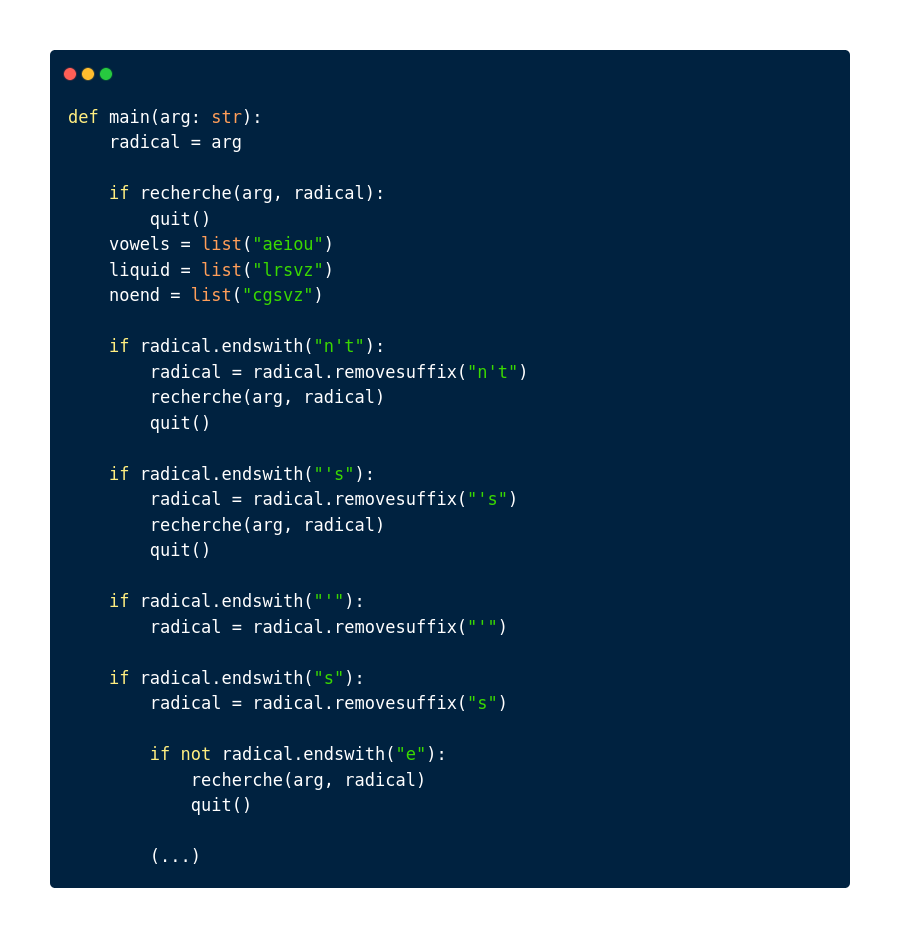
\includegraphics[scale=.23]{img/ex_morpho.png}

\end{figure}
\end{frame}

\section{Des outils plus efficaces : NLTK}


\begin{frame}{Retour de l'analyse morphologique de Terry Winograd}
\begin{figure}[ht]
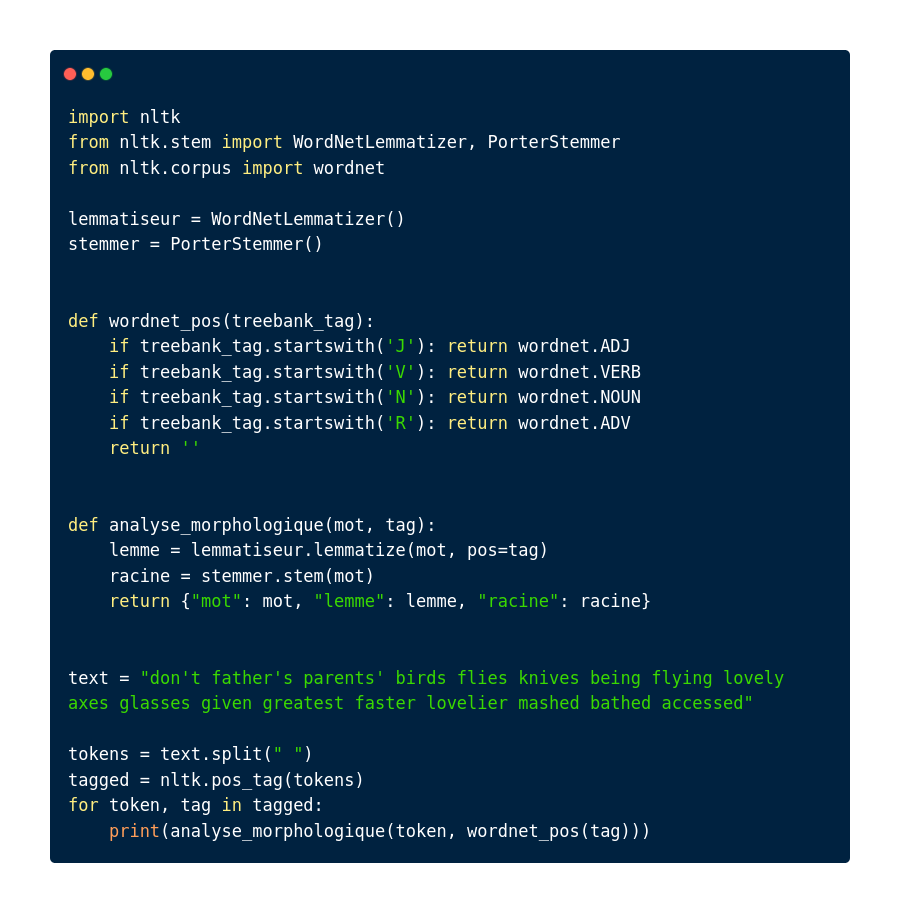
\includegraphics[scale=.24]{img/morpho_nltk.png}
\end{figure}
\end{frame}

\begin{frame}{Retour de l'analyse morphologique de Terry Winograd}
\begin{figure}[ht]
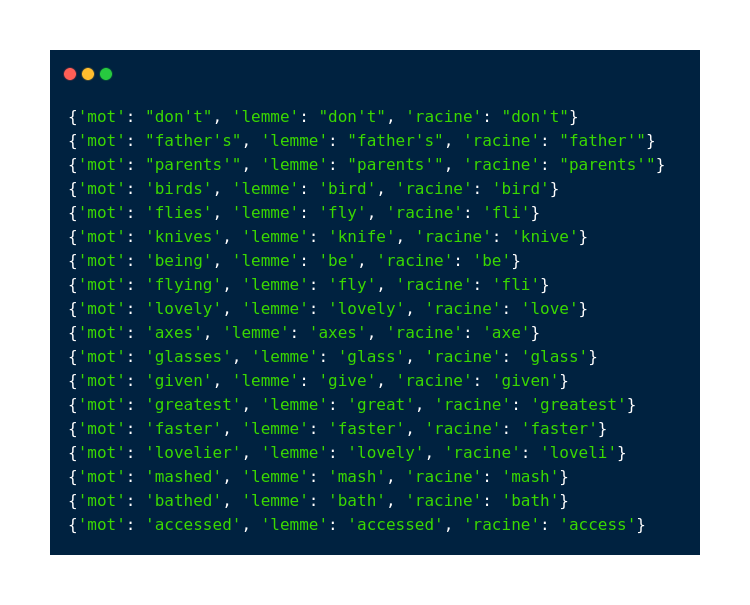
\includegraphics[scale=.24]{img/morpho_output_nltk.png}
\end{figure}
\end{frame}

\subsection{Analyse syntaxique}
\begin{frame}{\subsecname}
\begin{figure}[ht]
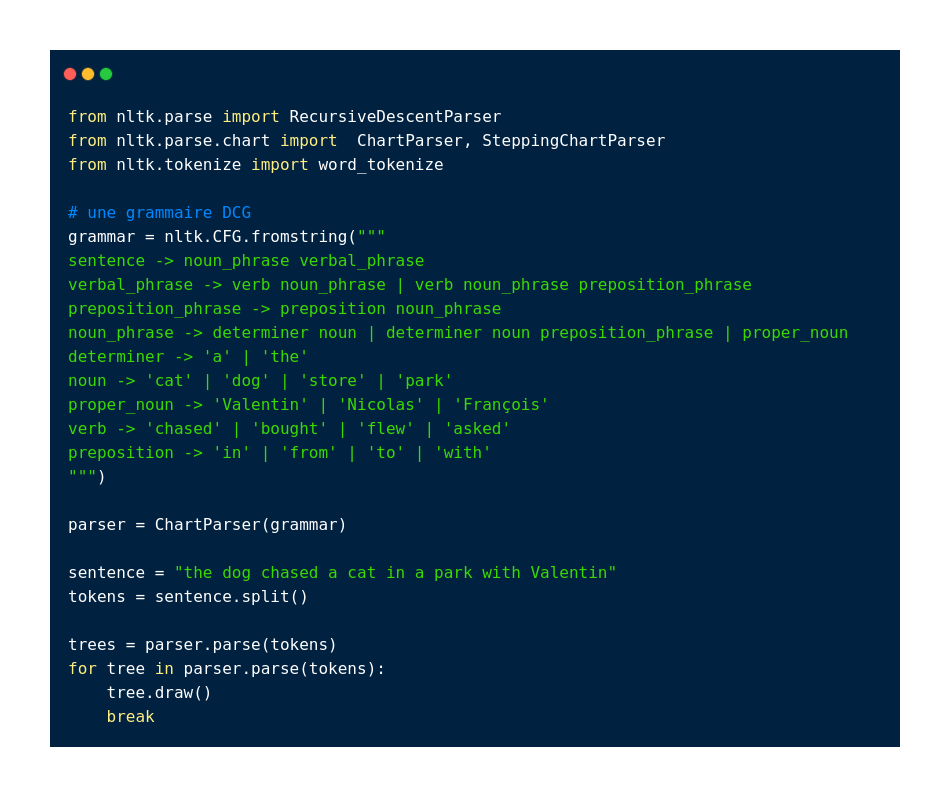
\includegraphics[scale=.25]{img/analyse_syntaxique_nltk.png}
\end{figure}
\end{frame}

\begin{frame}{\subsecname}
\begin{figure}[ht]
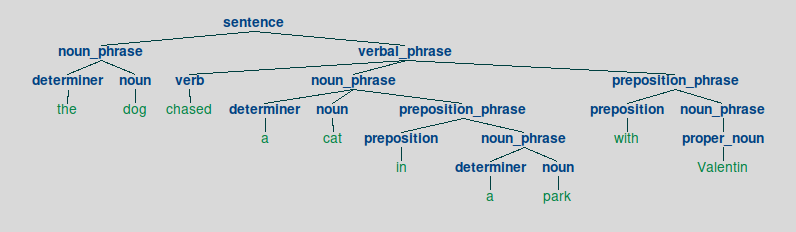
\includegraphics[scale=.4]{img/analyse_syntaxique_output_nltk.png}
\end{figure}
\end{frame}

\subsection{Named Entity Recognition}
\begin{frame}{\subsecname}

\begin{figure}[ht]

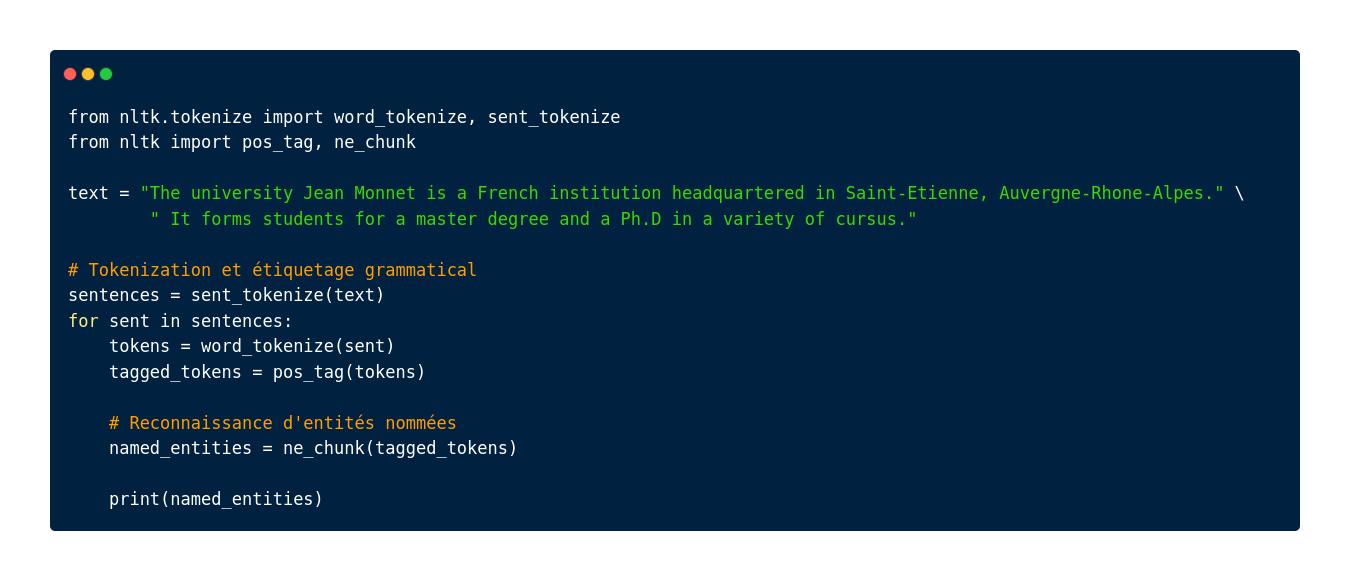
\includegraphics[scale=.22]{img/ner_nltk.png}
\end{figure}

\end{frame}

\begin{frame}{\subsecname}
\begin{figure}[ht]
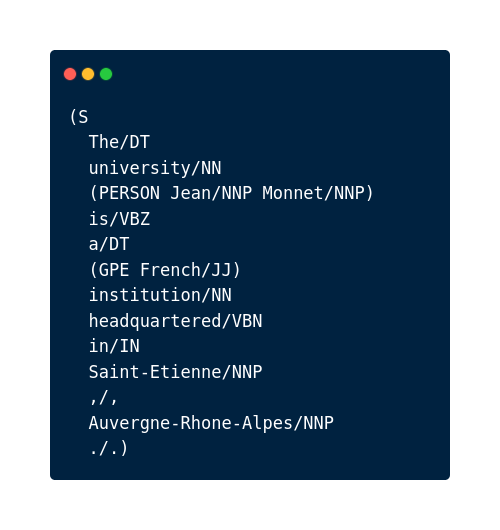
\includegraphics[scale=.3]{img/ner_output_nltk1.png}
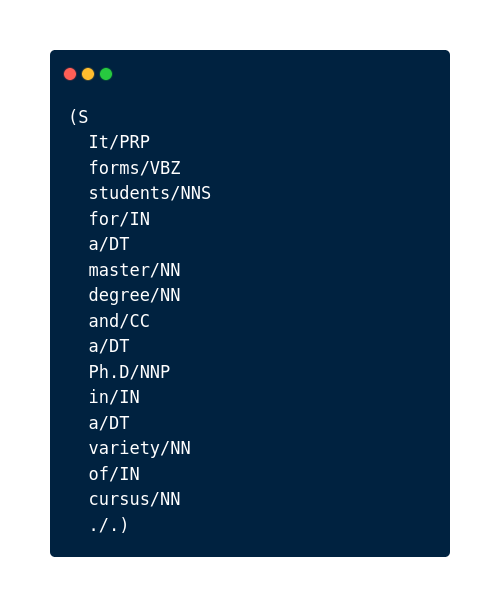
\includegraphics[scale=.3]{img/ner_output_nltk2.png}
\end{figure}
\end{frame}

\subsection{Analyse de similarité}

\begin{frame}{\subsecname}
\begin{figure}[ht]
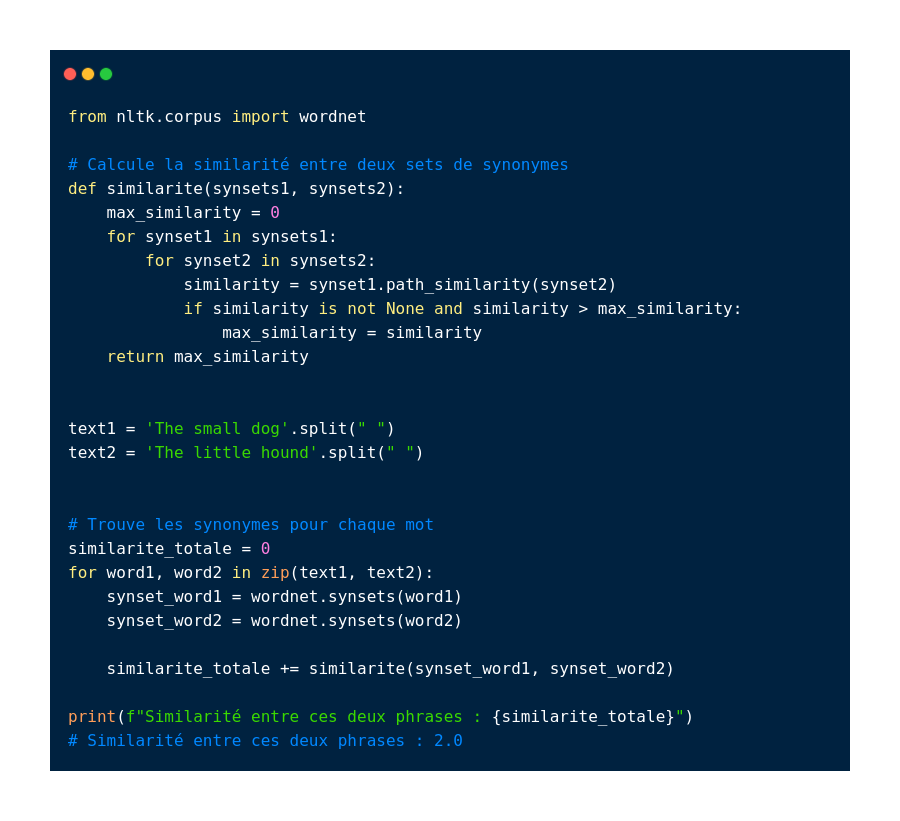
\includegraphics[scale=.26]{img/similarite_nltk.png}
\end{figure}
\end{frame}

\section{Machine Learning : classification et génération de texte}

\subsection{Classification de texte}

\begin{frame}{\subsecname}
\begin{figure}[ht]
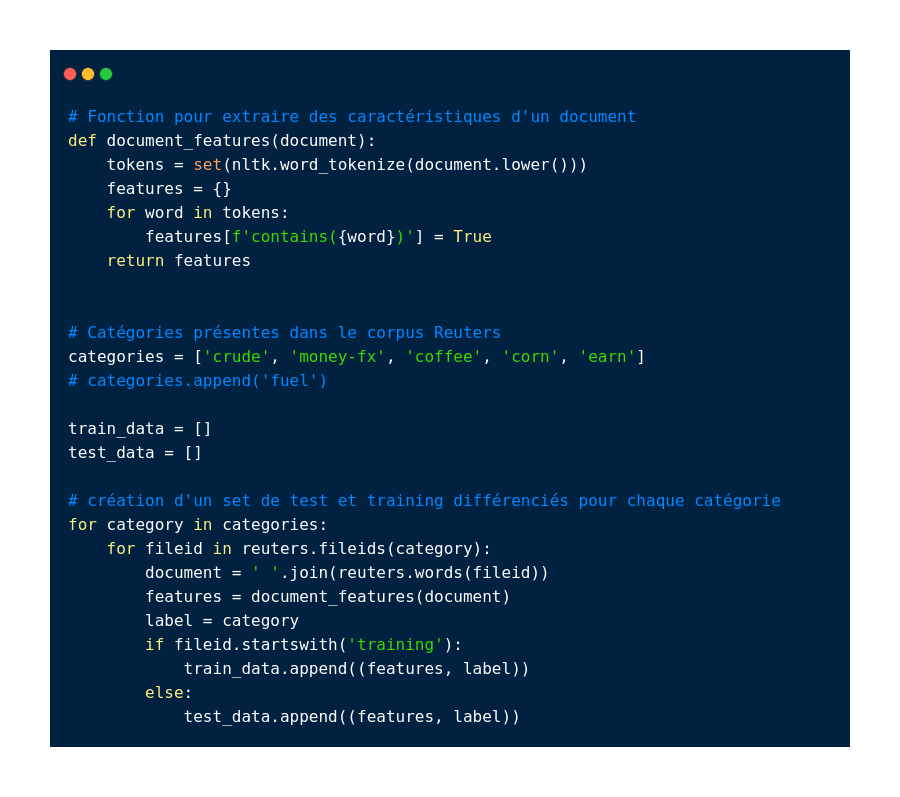
\includegraphics[scale=.27]{img/classifier1_nltk.png}

\end{figure}
\end{frame}

\begin{frame}{\subsecname}
\begin{figure}[ht]
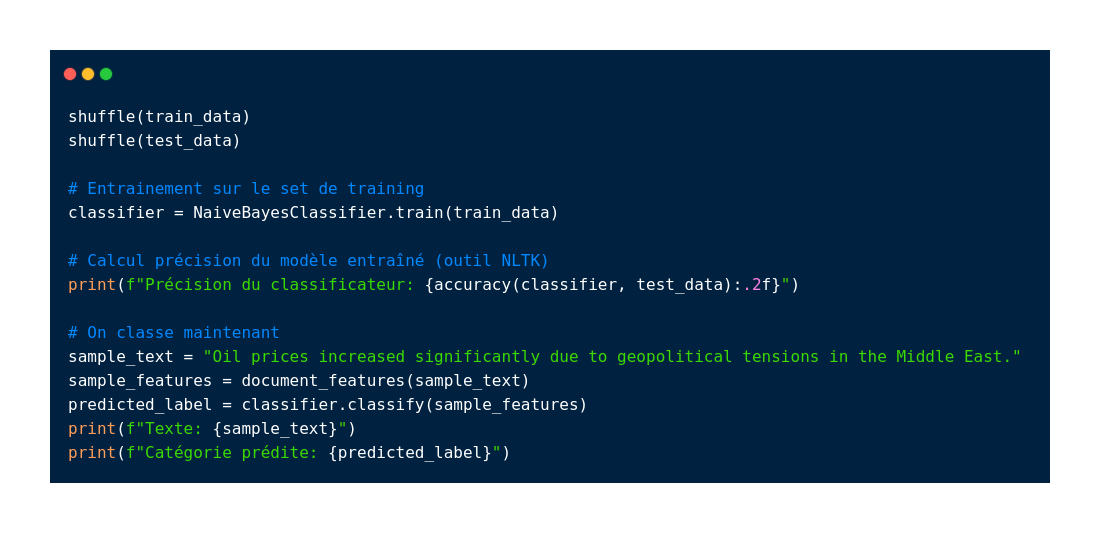
\includegraphics[scale=.29]{img/classifier2_nltk.png}
\end{figure}
\end{frame}

\begin{frame}{\subsecname}
\begin{figure}[ht]
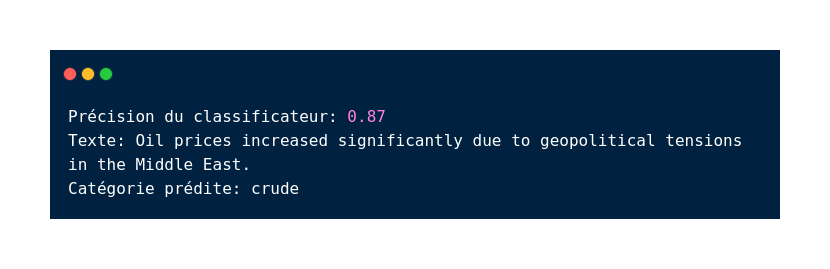
\includegraphics[scale=.36]{img/classifier_output_nltk.png}
\end{figure}
\end{frame}

\subsection{Analyse de sentiments}
\begin{frame}{\subsecname}
\begin{figure}[ht]
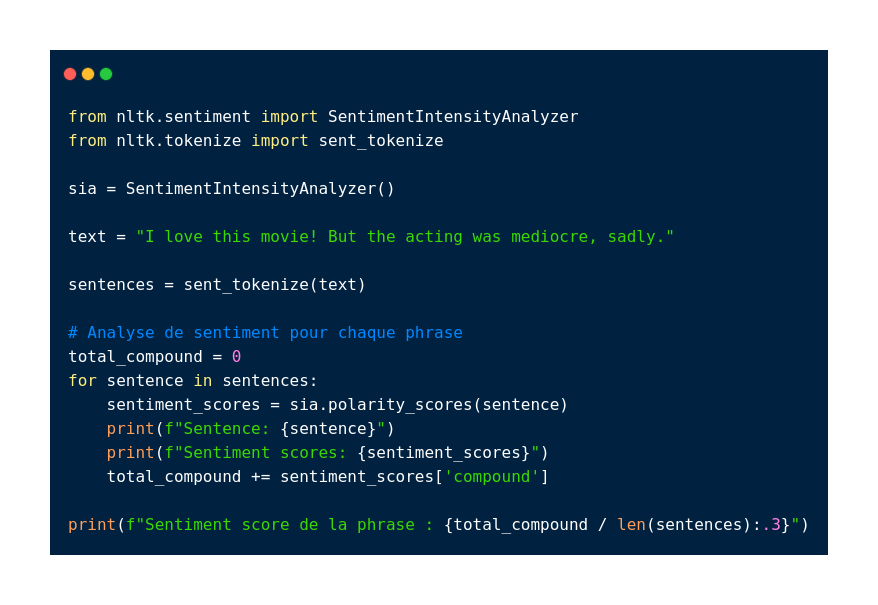
\includegraphics[scale=.32]{img/sentiment_nltk.png}

\end{figure}
\end{frame}

\begin{frame}{\subsecname}
\begin{figure}[ht]
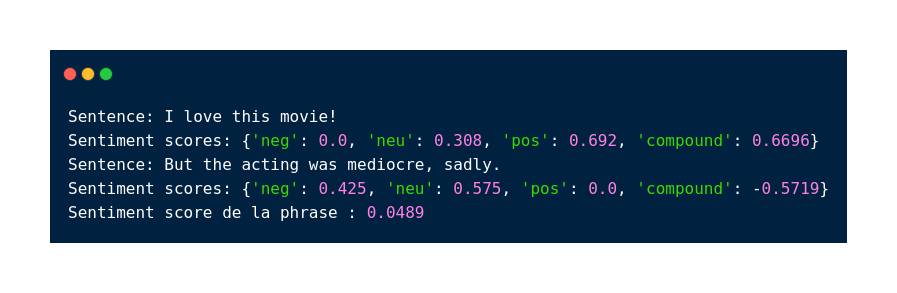
\includegraphics[scale=.32]{img/sentiment_output_nltk.png}
\end{figure}
\end{frame}

\subsection{Génération de texte}

\begin{frame}{\subsecname}
\begin{figure}[ht]
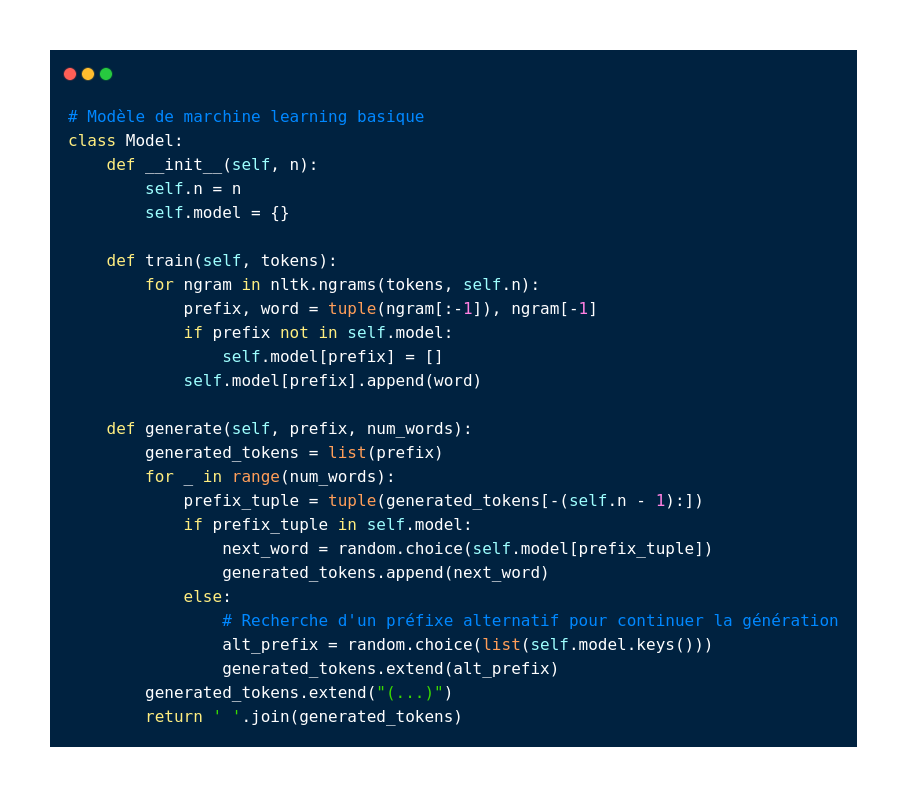
\includegraphics[scale=.27]{img/markov1_nltk.png}
\end{figure}
\end{frame}

\begin{frame}{\subsecname}
\begin{figure}[ht]
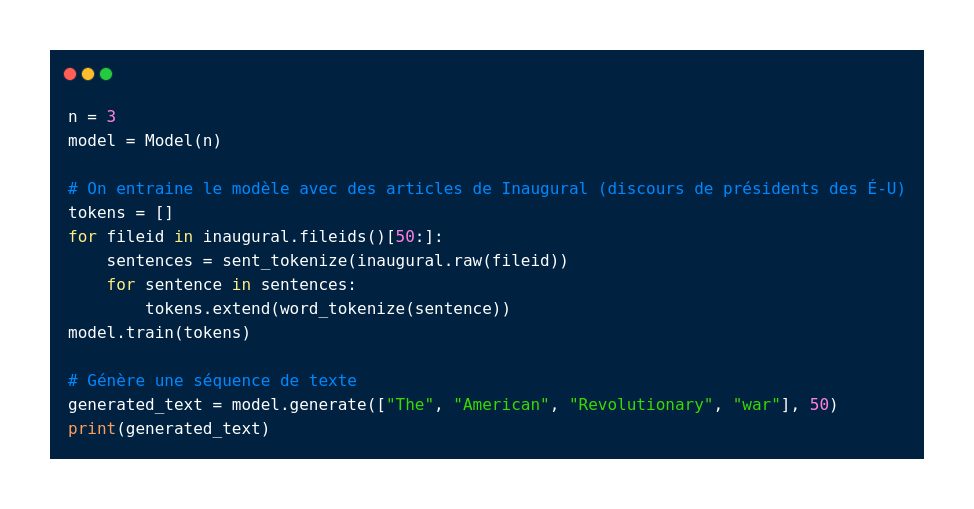
\includegraphics[scale=.31]{img/markov2_nltk.png}

\end{figure}
\end{frame}

\begin{frame}{\subsecname}
\begin{figure}[ht]
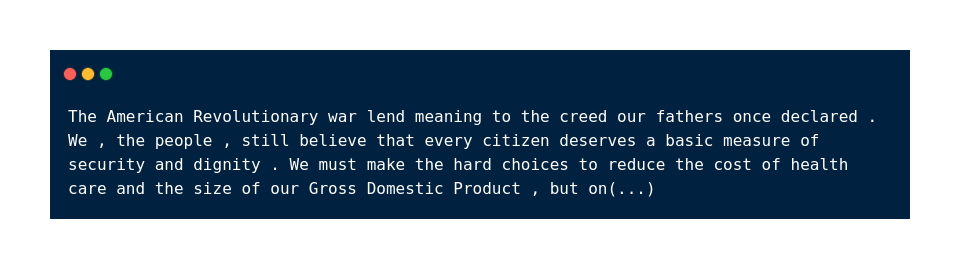
\includegraphics[scale=.33]{img/markov_output_nltk.png}
\end{figure}
\end{frame}

\section{Exemple : Prédiction d'évaluation}

\begin{frame}{Récupération des données}
\begin{figure}[ht]
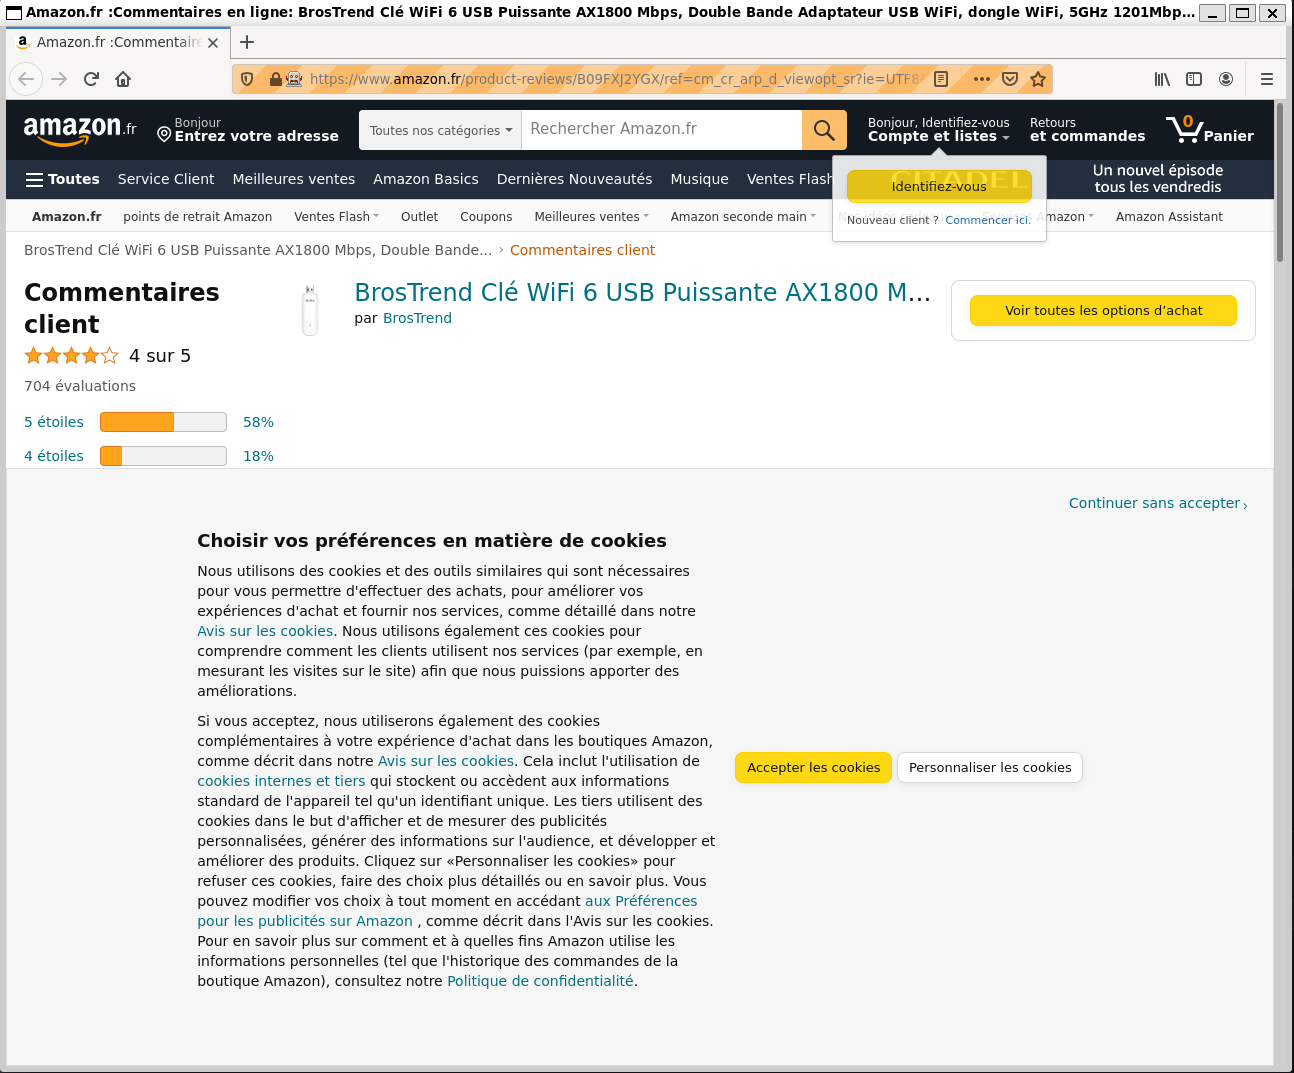
\includegraphics[scale=.23]{img/amazon.png}
\end{figure}
\end{frame}

\begin{frame}{Récupération des données}
\begin{figure}[ht]
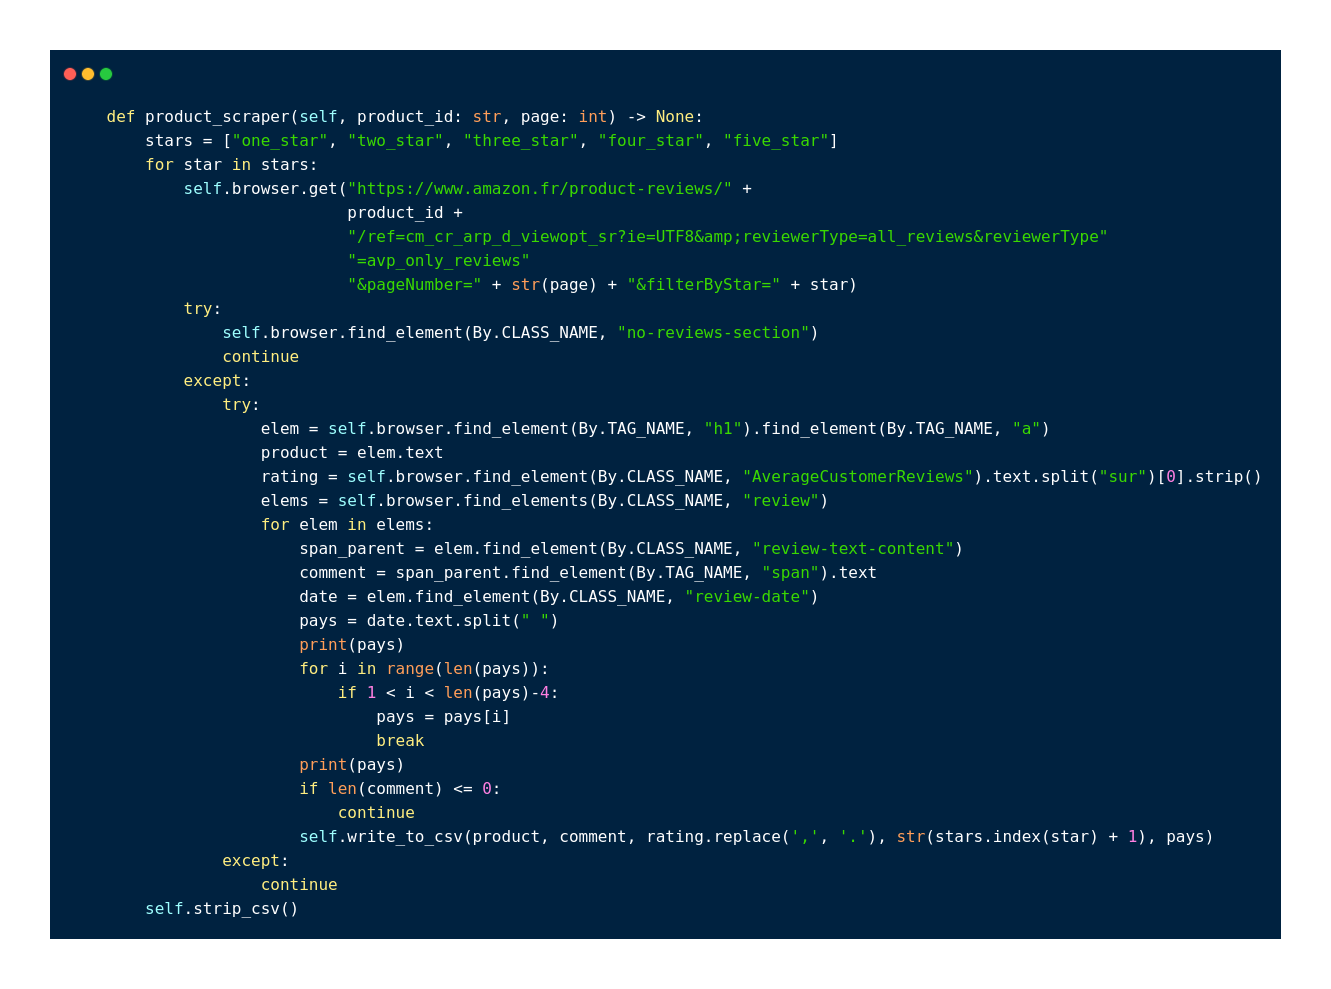
\includegraphics[scale=.22]{img/scraping_model.png}
\end{figure}
\end{frame}

\subsection{Analyse des données}

\begin{frame}{\subsecname}
\begin{figure}[ht]
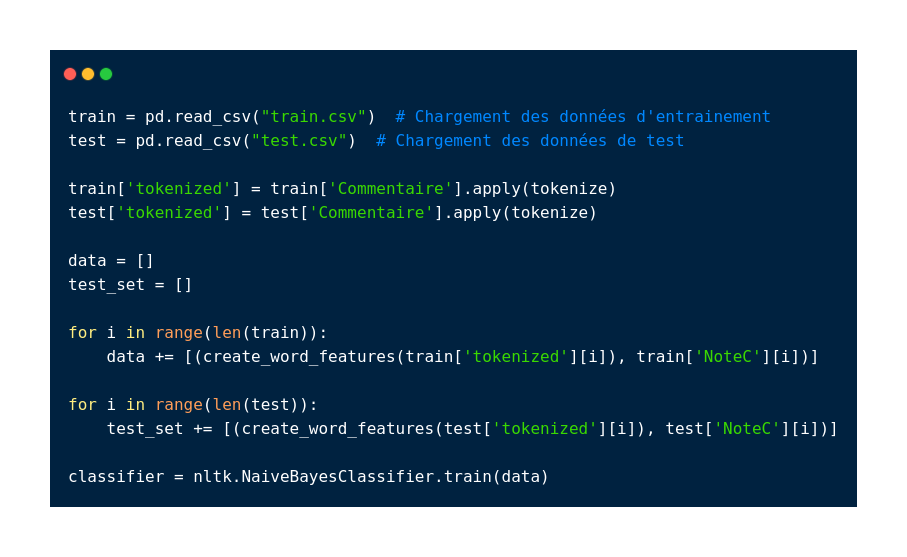
\includegraphics[scale=.3]{img/scraping_training.png}
\end{figure}
\end{frame}

\begin{frame}{\subsecname}
\begin{figure}[ht]
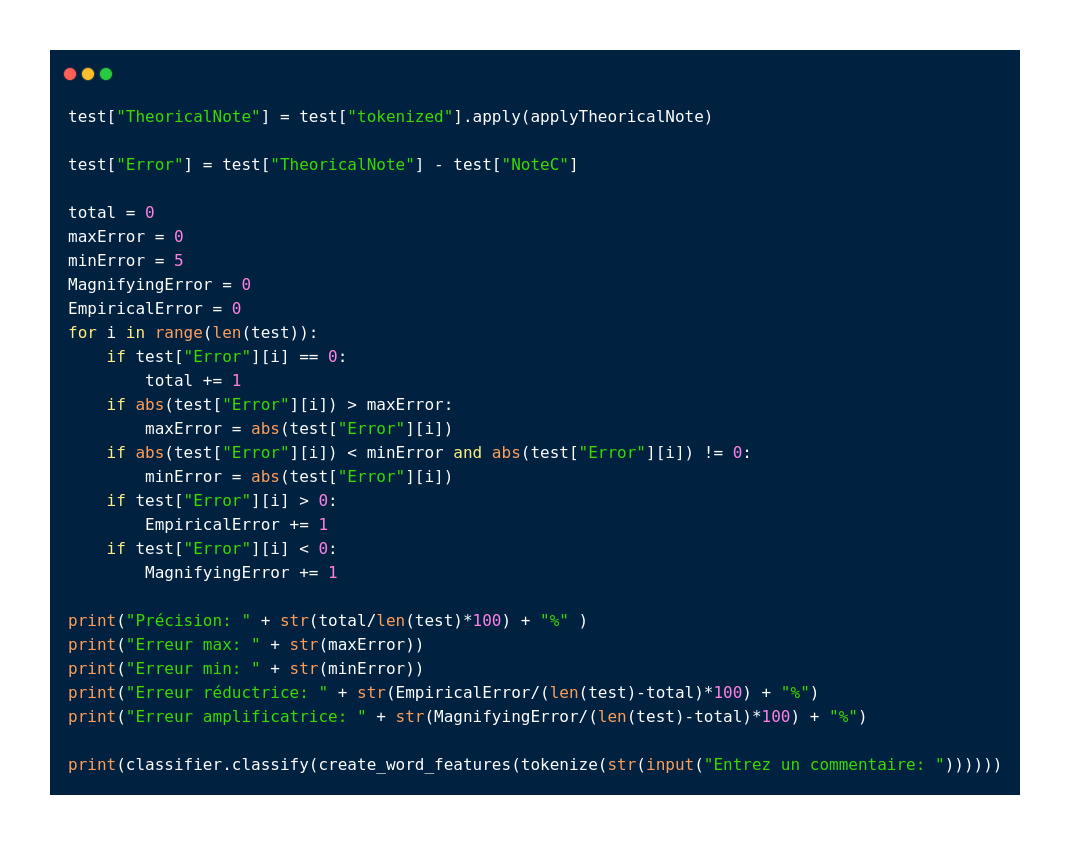
\includegraphics[scale=.25]{img/scraping_gathering.png}
\end{figure}
\end{frame}
\subsection{Résultats}
\begin{frame}{\subsecname}
\begin{figure}[ht]
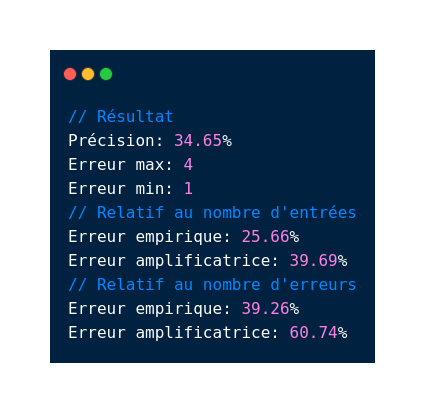
\includegraphics[scale=.34]{img/scraping_resultat.png}
\end{figure}
\end{frame}

\begin{frame}{\subsecname}
\begin{figure}[ht]
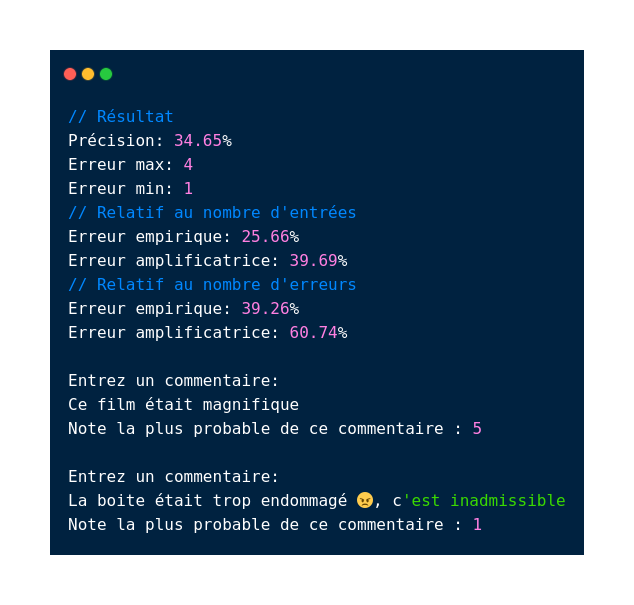
\includegraphics[scale=.3]{img/scraping_resultat2.png}
\end{figure}
\end{frame}

\section{Démonstration}

\section{Désavantages de NLTK}

\begin{frame}{\secname}
\begin{alertblock}{}
\begin{enumerate}[a)]
	\item "Anglo-centrisme"
	\item Obsolescence
	\item Deep Learning
\end{enumerate}
\end{alertblock}


\end{frame}

\section{Avantages de NLTK}

\begin{frame}{\secname}
\begin{alertblock}{}
\begin{enumerate}[a)]
	\item Praticité
	\item Quantité
	\item Corpus
	\item Open-source
\end{enumerate}
\end{alertblock}
\end{frame}

\begin{frame}{Sources}
	\begin{alertblock}{}
\begin{enumerate}[a)]
\item \textit{Natural Language Processing with Python,} \par \textit{Analyzing Text with the Natural Language Toolkit}
\item \textit{Stack Overflow}
\item \textit{codeimg.io}
\item \textit{github.com/nltk}
\end{enumerate}
\end{alertblock}
\end{frame}
\end{document}
